\documentclass[12pt, a4paper]{article} %mostra o tipo do documento
\setlength{\topmargin}{-.5in}
\setlength{\textheight}{9in}
\setlength{\textwidth}{6.3in}
\setlength{\oddsidemargin}{-.125in}
\setlength{\evensidemargin}{-.125in}
\usepackage[brazil]{babel} %permite escrever em português
\usepackage[utf8]{inputenc}
\usepackage[a4paper, textheight=260mm, textwidth=162mm]{geometry} %ajusta as margens
\usepackage[T1]{fontenc} %define a fonte das letras
\usepackage{color} %colore as letras
\usepackage{url} %inclui urls
\usepackage[pdfencoding=unicode]{hyperref} %transforma links em texto comum para clicar
\usepackage{amsmath, amssymb, amsthm, amsfonts} %permite fazer textos matemáticos
\usepackage{float} % permite mover tabelas e figuras para qualquer ponto da página
\usepackage{graphicx} %permite colocar imagens no documento

\title{Relatório EP2 - MAC0121}
\date{}
\author{João Gabriel Basi - $\text{N}^\circ$ USP: 9793801}
\begin{document}
\maketitle
\begin{enumerate}
\large
\item[1.]\textbf{O programa}
\normalsize\\[0.5cm]
Utiliza a técnica de backtracking para achar uma solução para o jogo de tabuleiro "Resta Um". O programa recebe as dimenções do tabuleiro e um matriz com 0, -1 e 1, representando sem buraco, buraco sem peça e buraco com peça respectivamente, e retorna os movimentos realizados para resolver o tabuleiro ou "Impossivel" se não há como resolvê-lo.\\
\large
\item[2.]\textbf{As funções}
\normalsize\\[0.5cm]
Foi criada uma struct chamada pilha que contém uma matriz, de número de linhas definido de acordo com o tabuleiro e 3 colunas, uma para guardar uma posição de linha, uma para posição coluna e a terceira para o movimento executado, além de duas variáveis inteiras, uma para guardar o topo da pilha e outra para guardar o tamanho máximo da pilha.\\
Foram criadas também algumas funções sobre essa struct:
\begin{itemize}
\item $criaPilha$: Aloca uma pilha de número de linhas especificado;
\item $pilhaVazia$: Verifica se a pilha está vazia;
\item $pilhaCheia$: Verifica se a pilha está cheia;
\item $empilha$: Empilha uma posição e um movimento na pilha;
\item $desempilha$: Desempilha a posição e o mivimento que estão no topo da pilha;
\item $imprimePilha$: Imprime as posições e movimentos guardados na pilha.
\end{itemize}
Foram criadas funções para ajudar na manipulação de matrizes:
\begin{itemize}
\item $criaMatriz$: Aloca uma matriz de número de linhas e colunas especificados;
\item $podeMexer$: Verifica se a peça pode ser movida e indica a direção do movimento;
\item $mexe$: Mexe ou volta uma peça.
\end{itemize}
Foram criadas algumas funções para verificações sobre matrizes:
\begin{itemize}
\item $concluido$: Verifica se as posições que estavam livres no começo estão ocupadas;
\item $ehPossivel$: Faz alguns testes (especificados no item 3) na distribuição das peças do tabuleiro para identificar se a distribuição pode ser resolvida;
\item $dfs$: Utilizada pela função $ehPossivel$ para verificar se o tabuleiro tem partes desconexas.
\end{itemize}
E, finalmente, algumas funções para resumir alguns processos:
\begin{itemize}
\item $criaVetor$: Aloca um vetor de tamanho especificado;
\item $freeAll$: Desaloca as estruturas alocadas na função main;
\item $freeAll2$: Desaloca as estruturas alocadas na função ehPossivel.\\
\end{itemize}
\large
\item[3.]\textbf{Conceitos matemáticos e simplificações utilizados}
\normalsize\\[0.5cm]
Na função $ehPossivel$ foram feitos três testes para identificar se um tabuleiro tem potencial para ser resolvido:
\begin{itemize}
\item O primeiro teste checa se $\text{N}^\circ$ de peças $\geqslant 2\cdot \text{N}^\circ$ de espaços iniciais, pois, para cada buraco sem peça do tabuleiro inicial é preciso de, no mínimo, um movimeto, e cada movimento precisa de duas peças para ser executado, então, se o tabuleiro tem $n$ buracos, é preciso de, pelo menos, $2n$ peças para resolvê-lo.
\item O segundo teste leva em conta a classe de posições do tabuleiro. Conforme foi descrito no site \url{http://recmath.org/pegsolitaire/index.html#pre}, a classe de posições do tabuleiro é definida enumerando as diagonais do tabuleiro do seguinte modo:\\
\begin{center}
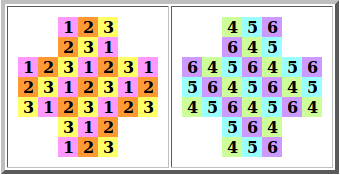
\includegraphics[scale=0.5]{peg_solitaire_classes.png}\\
Numeração no resta um tradicional
\end{center}
A partir disso, definimos uma função $N_i$ sobre o tabuleiro, que retorna a quantidade de casas ocupadas marcadas com número $i$, e a função $T$, que retorna o total de casas ocupadas. Com isso definimos a classe de posições do tabuleiro como sendo a 6-upla da forma $(T-N_1,T-N_2,T-N_3,T-N_4,T-N_5,T-N_6)\text{ }mod\text{ }2$ (no site é colocado como a "paridade" desses números, mas no programa eu considerei como módulo 2). Definidas as classes, observamos que a cada movimento executado a paridade dos númes dessa 6-upla não muda. Pegando como exemplo o tabuleiro da imagem, com a posição central livre e as outras ocupadas, vemos que, ao mexer qualquer peça para a posição central, os $N_2$ e $N_5$ aumentam em $1$ e os $N_1$, $N_3$, $N_4$, $N_6$ e $T$ diminuem em $1$, então, para os $N$s que diminuiram, temos que $N-1-(T-1)\equiv N-T\text{ }mod\text{ }2$, e para os que aumentaram $N+1-(T-1)\equiv N-T\text{ }mod\text{ }2$, vemos que essa regra vale para todo o tabuleiro e, concluimos que, a partir de um tabuleiro com certa classe de posição, só é possível atingir tabuleiros com a mesma classe, então temos que os tabuleiros final e inicial têm que estar na mesma classe, se não o tabuleiro é impossível. Lembrando que esse teste indicar que um tabuleiro é impossível é suficiente para que ele seja impossível, mas não é necessário.
\item O terceiro leva em conta a possibilidade de tabuleiros com partes desconexas, checando com a função $floodFill$ se, sempre quando há uma parte desconexa, ela tem no mínimo uma casa vazia, para que todas as peças possam ser movidas.\\[0.5cm]
\end {itemize}
\large
\item[4.]\textbf{Informações sobre os testes realizados}
\normalsize\\[0.5cm]
Considerando como núcleo a formação $3$x$3$ central do tabuleiro tradicional (imagem do item anterior) com a posição central livre e as outras ocupadas, e como braços as quatro partes restentes, escrevemos que um tabuleiro é $nnnn$ se tem o núcleo e $4$ braços $3$x$n$, contados a partir do de cima em sentido horário (notação encontrada no site citado no item 3).\\
\begin{itemize}
\item Testei com um tabuleiro $1111$, que passou nos testes da $ehPossivel$, mas, depois de $140seg$, o programa concluiu que ele é impossível;
\item Testei com o tabuleiro $2222$, que ele resolveu em pouco mais de $1seg$;
\item Testei com um tabuleiro $3322$, que passou no teste da $ehPossivel$, mas o programa não cconsiguiu achar uma resolução depois de meia hora rodando;
\item Testei para o tabuleiro francês, um tabuleiro com um núcleo $5$x$5$, e $4$ braços $3$x$1$ (também descrito no site ja citado) e o programa concluiu, ainda no teste das classes, que esse tabuleiro não é possível;
\item Testei com o tabuleiro $3333$ (clássico) e não foi resolvido depois de 3 horas\\[0.5cm]
\end{itemize}
\large
\item[5.]\textbf{Prós e contras}
\normalsize\\[-0.5cm]
\begin{itemize}
\item \textbf{Prós}\\[-0.5cm]
\begin{itemize}
\item Identifica boa parte dos tabuleiros que são impossíveis no começo do programa, deixando de gastar tempo tentando resolvê-los
\end{itemize}
\item \textbf{Contras}
\begin{itemize}
\item Não consegui dizer quais os melhores movimentos a serem feitos, então o programa demora para resolver tabuleiros grandes que possuem uma variedade pequena de soluções e tabuleiros que passaram nos pré-testes mas são impossíveis pois o algoritimo não está otimizado
\end{itemize}
\end{itemize}
\end{enumerate}
\end{document}